\subsection{Class diagram di design}
    \begin{flushleft}
        Verranno di seguito riportati i class diagram di design, che ora rispecchiano l'architettura del sistema e tutte le funzionalità nella loro
        interezza. \\
        \emph{\textbf{Nota}}: Tutti i costruttori banali (senza argomenti) e i getter e setter sono stati omessi per rendere più leggibili 
        i diagrammi
    \end{flushleft}

    \subsubsection{Login}
        \begin{figure}[H]
            \centering
            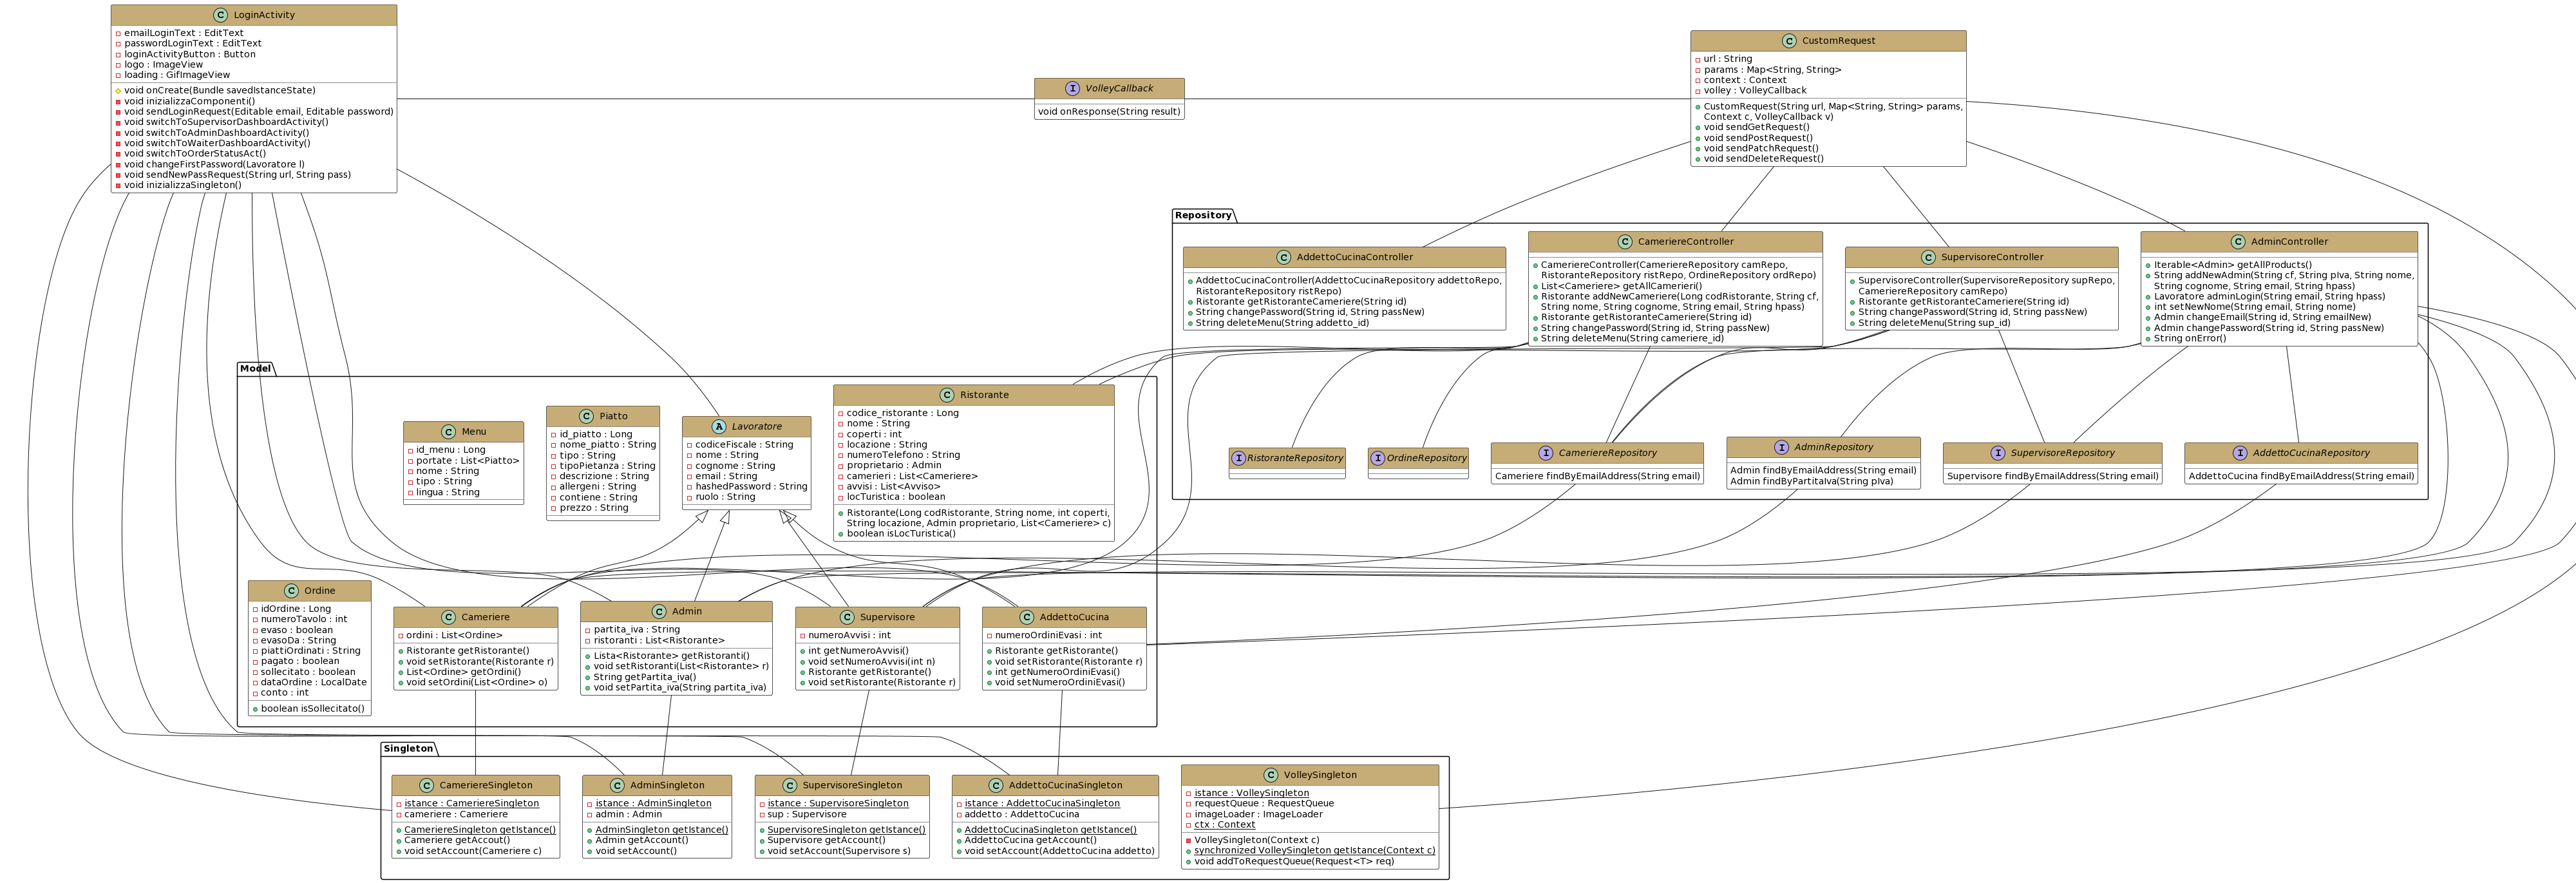
\includegraphics[scale=0.12]{assets/diagrammi/Class diagram di design/ClassDiagram_Login.png}
            \caption*{\textbf{CD01}:Class diagram Login}\label{fig:ClassDiagram_Login}
        \end{figure}


